\begin{chapter}{Konsensusmekanismien vertailu\label{vertailu}}
\begin{otherlanguage}{finnish}
Tämä kappale vertailee konsensusmekanismien kokonaisenergiankulutusta, yksittäisten siirtotapahtumien energiankulutusta sekä muita tärkeitä konsensusmekanismeihin liittyviä ominaispiirteitä, kuten skaalautuvuutta ja turvallisuutta. Vertailu tehdään käyttämällä teoriaosuudessa esiteltyjä merkittävimpiä lohkoketjuja esimerkkitapauksina kunkin konsensusmekanismin tyypillisestä energiankulutuksesta.

\begin{table}[!hbtp]
\begin{center}
\begin{tabular}{   | c |  c |  c |  c |   } 
  \hline
 \thead {Lohkoketjun \\ nimi} & \thead {Energiankulutus \\ (vuodessa)} & \thead {Transaktioita \\ sekunnissa (TPS)} & \thead {Energiankulutus \\ (siirtoa kohden)} \\ 
  \hline
 \makecell {Bitcoin (PoW)} & 200,57 TWh \cite{bitcoinenergy} & $\sim$7 \cite{bitcoin-tps} & 2006,54 kWh \\
  \hline
 \makecell {Ethereum (PoW)} & 94,73 TWh \cite{ethereumenergy} & $\sim$14 \cite{ethereum-tps} & 207,95 kWh \\
  \hline
 \makecell {Cardano (PoS)} & 6 GWh \cite{cardanoenergy} & $\sim$257 \cite{cardano-tps} & 0,5479 kWh  \\
  \hline
 \makecell {Algorand (PoS)} & 1,68 GWh \cite{algorand-energy} & $\sim$1300 \cite{algorand-energy-2} & 0,00534 kWh  \\
  \hline
 \makecell {Chia (PoSp)} & 0,307 TWh \cite{chiaenergy} & $\sim$20\footnotemark & 0,4864 kWh\footnotemark[\value{footnote}]  \\
  \hline
\end{tabular}
\caption{\label{tab:pow-database}Energiankulutus- ja sekunnissa tapahtuvien siirtotapahtumien vertailu eri lohkoketjujen välillä.}
\label{table-energy}
\end{center}
\end{table}

Taulukosta \ref{table-energy} huomataan, että PoW-lohkoketjujen vuosittainen energiankulutus on sekä PoS- että PoSp-konsensusmekanismeilla toimiviin lohkoketjuihin verrattuna merkittävästi suurempi. Vuosittainen energiankulutus on kuitenkin vertailukohteena harhaanjohtava, sillä sitä on hankala käyttää lohkoketjun energiatehokkuuden mittaamiseen. Täten taulukossa \ref{table-energy} on myös esitetty kuinka paljon energiaa yksi siirtotapahtuma vaatii.

\vspace{1cm}

\footnotetext{Siirtotapahtumien määrän on arvioitu olevan samaa luokkaa PoW-konsensusmekanismien kanssa. Ks. kappale \ref{chia}, missä esitetään millä menetelmällä Chian TPS ja energiankulutus siirtotapahtumaa kohden on arvioitu.}

Energiankulutusta vertailtaessa on lohkoketjujen markkina-arvolla myös merkittävä vaikutus niiden energiankulutukseen. Tyypillisesti matalan markkina-arvon lohkoketjut kuluttavat vähemmän energiaa, kun niissä on vähemmän solmuja ja louhijoita verrattuna suurempiin lohkoketjuihin. Kuvasta \ref{fig_energy} näkyy, miten lohkoketjun markkina-arvon noustessa sen energiankulutus kasvaa merkittävästi.

\begin{figure}[!ht]
\centering
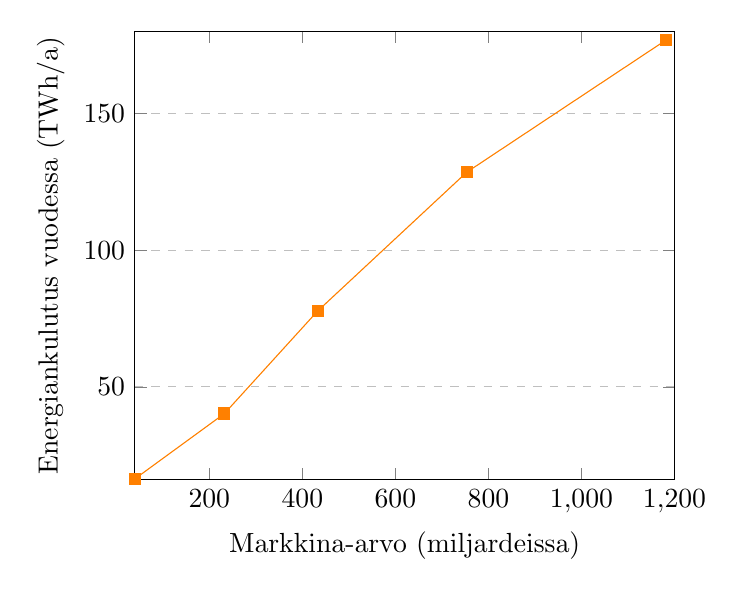
\begin{tikzpicture}
\begin{axis}[
    xlabel={Markkina-arvo (miljardeissa)},
    ylabel={Energiankulutus vuodessa (TWh/a)},
    xmin=40, xmax=1200,
    ymin=16, ymax=180,
    ymajorgrids=true,
    grid style=dashed,
]

\addplot[
    color=orange,
    mark=square*,
    ]
    coordinates {
    (40.15,16.37) % 01.09.2017: https://web.archive.org/web/20170901065814/https://digiconomist.net/bitcoin-energy-consumption
    (232.46,40.24) % 12.01.2018: https://web.archive.org/web/20180112215303/https://digiconomist.net/bitcoin-energy-consumption
    (433.04,77.78) %  24.12.2020: https://web.archive.org/web/20201224110206/https://digiconomist.net/bitcoin-energy-consumption
    (753.24,128.51) % 15.06.2021: https://web.archive.org/web/20210615053124/https://digiconomist.net/bitcoin-energy-consumption
    (1181.3,176.83) % 19.10.2021: https://web.archive.org/web/20211019194409/https://digiconomist.net/bitcoin-energy-consumption
    };
    
\end{axis}
\end{tikzpicture}
\caption{Bitcoinin energiankulutus markkina-arvon kasvaessa. Kuvaajan tilastot on kerätty ottamalla sen markkina-arvo Coingecko-verkkosivulta \cite{Coingecko} ja samalta päivältä sen energiankulutus Digiconomist-verkkosivun energiankulutustilastosta Waybackmachinella\footnotemark}
\label{fig_energy}
\end{figure}

\footnotetext{
\begin{scriptsize}
\url{https://web.archive.org/web/20170901065814/https://digiconomist.net/bitcoin-energy-consumption} \\
\url{https://web.archive.org/web/20180112215303/https://digiconomist.net/bitcoin-energy-consumption} \\
\url{https://web.archive.org/web/20201224110206/https://digiconomist.net/bitcoin-energy-consumption} \\
\url{https://web.archive.org/web/20210615053124/https://digiconomist.net/bitcoin-energy-consumption} \\
\url{https://web.archive.org/web/20211019194409/https://digiconomist.net/bitcoin-energy-consumption}
\end{scriptsize}
}

Energiankulutuksen kasvu markkina-arvon kasvaessa kuvan \ref{fig_energy} esittämällä tavalla pätee vain PoW-konsensusmekanismilla toimiviin lohkoketjuihin. PoS:ssä solmujen määrä ei kasva yhtä merkittävästi markkina-arvon kasvaessa, sillä PoS:ssä osakkaiden ja sijoitetun pääoman määrä kasvaa vastaavalla tavalla, mutta solmujen ylläpito ei ole yhtä kannattavaa käyttäjälle. PoSp:ssä puolestaan on esitetty, että lohkoketjun vaatima tallennustilan määrä voi kasvaa vastaavalla tavalla, mutta tallennustilan ollessa energiankulutukseltaan huomattavasti tehokkaampaa ei energiankulutus kasva yhtä merkittävästi.

Tutkielma vertailee seuraavaksi teemoittain konsensusmekanismien ongelma-alueita. Teemat ovat energiankulutus, elektroniikkajäte, hiilidioksidipäästöt, skaalautuvuus ja hajautuneisuus. Hajautuneisuutta vertailtaessa tutkielma käsittelee myös konsensusmekanismien turvallisuutta.

\begin{section}{Energiankulutus\label{energiankulutus}}

Proof-of-Work (PoW) on taulukon \ref{table-energy} perusteella energiankulutukseltaan ongelmallisin. Ekologiselta kannalta tarkasteltuna PoW-lohkoketjut jo pelkän vaatimansa energian takia eivät ole kestäviä. Kuvaajasta \ref{fig_energy} huomataan, että niiden energiankulutus tulee vain jatkamaan kasvuaan mitä suuremmaksi lohkoketjujen markkina-arvo kasvaa. Tämä energiakulutuksen kasvaminen lohkoketjun markkina-arvon nousun myötä selittyy sillä, että kalliimpaa kryptovaluuttaa voidaan louhia suuremmalla energiankulutuksella ilman, että louhinnasta tulee epäkannattavaa. Mikäli kryptovaluutan hinta laskee joutuu puolestaan osa louhijoista lopettamaan louhimisen, sillä louhinnasta saadut palkkiot eivät enää riitä maksamaan sähkökuluja.

Proof-of-Space (PoSp) pärjää vertailussa huomattavasti paremmin, ja yhtä siirtotapahtumaa kohden vie vähemmän energiaa kuin Cardano. Kuitenkin Chian markkina-arvon ollessa 0,021\% Bitcoinin markkina-arvosta ja 0,48\% Cardanon markkina-arvosta joulukuussa 2021 \cite{Coingecko}, voidaan olettaa lohkoketjun energiankulutuksen sen markkina-arvon kasvaessa nousevan vielä huomattavasti suuremmaksi. Tilastossa on kuitenkin huomioitava se, että Chian energiankulutus siirtotapahtumaa kohden on arvioitu sen mukaan, mikäli lohkoketju toimisi sen maksimikapasiteetilla siirtotapahtumien käsittelyssä sekunnissa. Todellisuudessa Chia käsittelee huomattavasti vähemmän siirtotapahtumia sekunnissa, ja näin ollen energiankulutus siirtotapahtumaa kohden on tilastoissa ilmoitettua lukua suurempi.

Proof-of-Stake (PoS) on vertailussa energiankulutukseltaan tehokkain. Ottaen huomioon, että Cardano on markkina-arvoltaan kuudenneksi suurin, ja kuluttaa silti vain 0,5479 kilowattia yhtä siirtotapahtumaa kohden, suoriutuu se tehokkuusvertailussa hyvin. Algorandin energiankulutus siirtotapahtumaa kohden on vain 0,00534 kilowattituntia, mikä on huomattavasti vähemmän kuin minkään muun vertailtavan lohkoketjun. Tämä korkea energiatehokkuus selittyy sillä, että Algorand käsittelee paljon enemmän siirtotapahtumia sekunnissa kuin muut vertailtavat lohkoketjut \cite{algorand-energy-2}. Algorand käyttää myös tapahtuman varmentamiseen vain hieman yli sataa \cite{algorand-energy} varmentajasolmua, mikä näkyy energiatehokkuutena, mutta vastaavasti voi vaikuttaa negatiivisesti lohkoketjun turvallisuuteen ja hajautuneisuuteen.

\end{section}
\section{Elektroniikkajäte\label{elektroniikkajate}}
\begin{otherlanguage}{english}

PoW on elektroniikkajätteen kannalta ongelmallinen. PoW:ssa kaupallisesti kannattavaan louhintaan soveltuu ainoastaan siihen erikoistuneet laitteet (ASIC, Application Specific Integrated Circuit), jotka kaikki joudutaan korvaamaan uudemmilla laitteilla kahden vuoden välein \cite{btc-carbon-ewaste}. Käytöstä poistuvat laitteet tuottavat suuren määrän elektronista jätettä: kesäkuun 2019 ja kesäkuun 2020 välillä Bitcoinin arvioitiin tuottaneen 27,1 kilotonnia elektronista jätettä. Suomi tuotti vuonna 2019 noin 110 kilotonnia elektronista jätettä \cite{ewaste-finland}, johon suhteutettuna Bitcoin vastaisi noin 24,6\% Suomen samaan aikaan tuottamasta elektronisesta jätteestä. Bitcoin-louhijoita mininpoolstats.com-verkkosivun tilastojen mukaan on noin 5,11 miljoonaa \cite{btc-pool-stats-miner-count}.

PoS on puolestaan elektroniikkajätteen määrää vertailtaessa hyvä. PoS-lohkoketjujen elektroniikkajäte tulee solmuja ylläpitävistä tietokoneista. Solmujen määrä on tämän tutkielman käsittelemissä lohkoketuissa, eli Cardanossa ja Algorandissa, silti verrattuna PoW- ja PoSp:n louhijoihin varsin pieni. Cardanolla on joulukuussa 2021 noin 4700 osakkuusallasta \cite{cardano-staking-pools}, mistä voidaan arvioida solmuja olevan suunnilleen saman verran, kun solmut ylläpitävät osakkuusaltaita. Algorandin tilastossa joulukuussa 2021 solmuja on noin 1500 \cite{algorand-tps-nodes-etc}. Hyvin optimoiduissa PoS-lohkoketjuissa solmu vaatii vain tyypillisen kuluttajatason tietokoneen toimiakseen. Solmun ylläpitäminen hyvin optimoidussa PoS-lohkoketjussa ei ole laitteistolle normaalia käyttöä kuluttavampaa, sillä PoS-solmujen ylläpito ei vaadi prosessorin jatkuvaa rasittamista tai jatkuvaa lukemista kovalevyltä. Tämän vuoksi PoS-laitteisto kestää käyttöä pidempään, eikä laitteistoa tule jatkuvasti päivittää paremmaksi säilyttääkseen kilpailukykyisyyden.

PoSp:ssä on miningpoolstats.com-verkkosivun mukaan louhijoita 209 tuhatta joulukuussa 2021 \cite{chia-pool-stats}. PoS:n verrattuna lohkoketjua ylläpitäviä laitteita on jo huomattavasti enemmän. PoSp:n aiheuttama kulutus laitteiden kovalevyille on kiistelty, eikä siitä ole tehty tarkkoja tutkimuksia. Osa käyttäjistä on kuitenkin raportoinut esimerkiksi SSD:n hajoavan käytössä jo muutaman kuukauden sisällä. Tämän lisäksi Chia aiheutti julkaisunsa aikana uusien kovalevyjen myynnin kasvua, ja mikäli Chia kuluttaa saman verran kovalevyjä kuin tyypilliset kaupallisessa käytössä olevat serverit, on niiden elinikä noin neljä vuotta \cite{manufacturingcarbon1}.

Chia kuitenkin eroaa kaupallisista serveritietokoneista siinä, että Chiassa kovalevyille ei tallenneta mitään kriittistä dataa. Tällöin tallennuslaitteita voidaan käyttää niiden hajoamiseen saakka. On siis mahdollista, että Chian louhijat ostaisivat käytettyjä kovalevyjä esimerkiksi kaupallisten servereiden luopuessa niistä takuuajan umpeuduttua. Tällöin Chia edistäisi tallennuslaitteiden kierrättämistä ja toimisi suureksi osaksi tallennuslaitteiden elinkaaren loppusijoituskohteena. Kovalevyjen kysynnän ja hinnan kasvaessa tällainen tilanne on etenkin mahdollinen, sillä toisin kuin PoW:ssa, Chiassa louhintaa voi tehdä normaalilla kuluttajatason laitteella, eikä ASIC:n käyttö ole tarpeellista.

\end{otherlanguage}
\begin{section}{Hiilidioksidipäästöt\label{hiilidioksidipaastot}}

PoW on hiilidioksidipäästöjen osalta konsensusmekanismeista suurin saastuttaja. Energiankulutuksen ja louhintaan erikoistuneiden laitteiden valmistamisen arvioitiin vuonna 2019 aiheuttaneen kokonaisuudessaan 39,27 megatonnia hiilidioksidipäästöjä Bitcoinin osalta \cite{btc-carbon-ewaste}. Suomen laskettiin vuonna 2019 aiheuttaneen 42,55 megatonnia hiilidioksidipäästöjä \cite{carbon-finland}, eli Bitcoin vastaa miltei Suomen vuosittaista hiilijalanjälkeä. Ethereumin vaatiessa vastaavanlaista erikoistunutta laitteistoa ja sen energiankulutuksen ollessa noin puolet siitä miten paljon Bitcoin tällä hetkellä vaatii energiaa vuodessa, voidaan arvioida Ethereumin hiilijalanjäljen olevan noin puolet Bitcoinin hiilijalanjäljestä.

Hiilidioksidipäästöjen laskeminen PoSp:lle on huomattavasti hankalampaa, sillä aihetta ei ole vielä tutkittu. Kovalevyjen valmistamisen arvioitiin Euroopan unionin komission toimesta vaativan noin kaksi kilowattituntia energiaa \cite{manufacturingcarbon1}, mutta on hankalaa arvioida kuinka moni Chian louhijoista ostaa uusia kovalevyjä louhintaan. Energiankulutuksesta voidaan kuitenkin laskea, että kun De Loosen ja kollegoiden tutkimuksessa \cite{btc-carbon-ewaste} esitetyn arvion mukaan kryptolouhinta aiheuttaa keskimäärin \(473.64~g~CO_{2}/kWh \), aiheuttaisi Chia 0,1454 megatonnia hiilidioksidipäästöjä vuodessa.

PoS:n energiankulutuksen ollessa vuosittain vain joitakin gigawattitunteja ja kun PoS ei aiheuta merkittävää uusien laitteiden ostamista ja näin ollen elektroniikkajätettä, sen hiilidioksidipäästöt ovat marginaaliset sekä PoW:n että PoSp:n verrattuna.

\end{section}
\begin{section}{Skaalautuvuus\label{skaalautuvuus}}

PoW-lohkoketjut ja PoSp-lohkoketjuna Chia häviävät PoS-lohkoketuille siirtotapahtumien määrässä sekunnissa. Taulukon \ref{table-energy} mukaan Bitcoin kykenee ainoastaan seitsemään siirtotapahtumaan sekunnissa, kun taas Ethereum pystyy suorittamaan 14 siirtotapahtumaa sekunnissa. Chian on arvioitu pystyvän suorittamaan noin 20 siirtotapahtumaa sekunnissa. Kun lohkoketjut pystyvät suorittamaan vain hyvin rajallisen määrän siirtoja sekunnissa, on tyypillistä että siirtotapahtumien käsittelyssä menee kauan ja lohkoketju voi ruuhkautua niin, että siirtotapahtumat eivät suoritu lainkaan. Mikäli lohkoketjujen pyrkimyksenä on toimia globaalina virtuaalivaluuttana vaaditaan tehokkaampia ratkaisuja. PoW-lohkoketjuja on kuitenkin mahdollista skaalata nostamalla niiden lohkojen kokoa (eng. \textit{block size}), mikä puolestaan vaatii tehokkaampia solmuja. Tästä syystä tässä tutkielmassa vertailtavat PoW- ja PoSp-lohkoketjut ovat päätyneet lohkoketjun tasa-arvoisuuden ja hajautuneisuuden kannalta siihen tulokseen, että ihanteellinen siirtotapahtumien määrä sekunnissa on noin kaksikymmentä. Mikäli PoW- ja PoSp-lohkoketjut nostaisivat lohkojensa kokoa, joutuisvat useat solmut lopettaa toimintansa laitteistovaatimuksien kasvaessa. Korkeat laitteistovaatimukset saattaisivat myös näkyä suurempana energiankulutuksena. PoW- ja PoSp-lohkoketjut käyttävätkin skaalaamiseensa tyypillisesti layer-2 ratkaisuja.

PoS-lohkoketjuista Cardano ylittää PoW- ja PoSp-lohkoketjujen siirtotapahtumien määrän sekunnissa yli kymmenkertaisesti. Algorand puolestaan ylittää Bitcoinin siirtotapahtumien määrän sekunnissa yli satakertaisesti, ja pärjää vertailussa parhaiten. Näiden lukujen perusteella PoS on konsensusmekanismeista skaalautuvin.

PoW- ja PoSp-lohkoketjuihin on kuitenkin esitetty niiden skaalautuvuuden ratkaisemiseksi jo aikaisemmin mainittuja layer-2 ratkaisuja. Näissä ratkaisussa lohkoketjulle rakennetaan rinnakkaisia lohkoketjuja, missä voidaan suorittaa siirtoja rinnakkaisesti päälohkoketjun, eli niin kutsun layer-1:n kanssa. Layer-2 ratkaisut jakavat päälohkoketjunsa konsensusmekanismin tavallisesti hyödyntämällä älysopimuksia, ja tällä tavoin pystyvät hyödyntämään päälohkoketjun tarjoamaa turvallisuutta. Esimerkiksi Ethereumia on tällä tavoin jo skaalattu Arbitrum- ja Optimism layer-2 ratkaisuilla. Samanlainen ratkaisu pystytään kuitenkin tekemään myös PoS-lohkoketjuissa, ja Cardano on arvioinut pystyvänsä layer-2 ratkaisulla skaalamaan siirtotapahtumien määrää sekunnissa yli miljoonaan \cite{cardano-hydra}. Layer-2 ratkaisujen lisäksi esimerkiksi Ethereumia on jo skaalattu myös sivuketjuilla (eng. \textit{sidechains}), kuten Polygonilla. Sivuketjut eroavat layer-2 ratkaisuista siinä, että ne ovat päälohkoketjusta täysin irrallisia lohkoketjuja, joilla on oma konsensusmekanismi ja tyypillisesti myös oma kryptovaluuttansa. Layer-2 ratkaisuilla ja sivulohkoketjuilla voi mahdollisesti olla merkittäviä energiankulutus- ja ympäristövaikutuksia, mutta näistä on toistaiseksi hyvin vähän tutkimustietoa.

Keskitetyt kryptovaluutanvaihtopalvelut, kuten Binance ja Coinbase, helpottavat myös lohkoketjujen ruuhkautumista. Mikäli kryptovaluuttaa siirretään keskitetyissä vaihdantapalveluissa, ei tällaiset siirrot tapahdu lohkoketjussa itsessään. Kryptovaluuttaa voi myös siirtää muissa lohkoketjuissa, ja tällaisia ratkaisuja on esimerkiksi Wrapped Bitcoin. Wrapped Bitcoinissa myönnetään Bitcoinia vastaava niin kutsuttu wrapped-kolikko, jota voidaan natiivisti siirtää esimerkiksi Ethereumissa tai muissa lohkoketjuissa käyttäjien välillä. Wrapped-kolikot voi halutessaan muuntaa takaisin Bitcoiniksi. Sekä keskitetyt vaihdantapalvelut että wrapped-kolikot vaativat kuitenkin jonkin erillisen tahon, johon käyttäjien täytyy luottaa. Tällöin kryptovaluuttojen ajatus luottamuksettomasta valuutasta kärsii.

Skaalautuvuuden vertailu lohkoketjujen välillä on ongelmallista, sillä kaikkia vertailussa olevia lohkoketjuja on mahdollista skaalata. PoW- ja PoSp-lohkoketjut pärjäävät huonosti vertailussa, mutta niitä voitaisiin skaalata hyvinkin yksinkertaisesti lohkojen kokoa nostamalla. Kuitenkin näiden lohkoketjujen suurimmaksi eduksi usein mainitaan niiden korkea hajautuneisuus, mikä kärsisi tällaisesta muutoksesta merkittävästi. Lohkoketjuja onkin täten mielekkäämpää skaalata esimerkiksi sivulohkoketjuilla ja layer-2 ratkaisuilla, mitkä eivät vaikuta lohkoketjujen hajautuneisuuteen negatiivisesti, ja PoW-lohkoketjuja onkin jo skaalattu tällaisilla ratkaisuilla. Skaalamisen vaikutuksista energiankulutukseen ei ole vielä olemassa merkittäviä tutkimuksia ja sen aiheuttamat muut ympäristöongelmat ovat toistaiseksi epäselvät, mikä vaikeuttaa skaalautuvuuden vertailua tutkielman ekologisuuskeskeisessä kontekstissa.

\end{section}
\section{Hajautuneisuus\label{hajautuneisuus}}
\begin{otherlanguage}{english}

Tyypillisesti konsensusmekanismeja vertailtaessa esitetään PoW:n eduksi sen hajautuneisuus, ja samaa on esitetty myös PoSp:n eduksi. Vaikka PoW:ssa ja PoSp:ssa on huomattavia ympäristöongelmia verrattuna PoS:n, on niitä oikeutettu sillä ettei PoS ole todellisesti hajautettu. Cardanossa esimerkiksi joulukuussa 2021 on noin 4700 osakkuusallasta (staking pool) \cite{cardano-staking-pools} ja Algorandissa solmuja on noin 1500 \cite{algorand-tps-nodes-etc}. Bitcoinissa louhijoita on yli viisi miljoonaa \cite{btc-pool-stats-miner-count}, mutta louhinta jakautuu yhteensä kolmentoista suuren louhinta-altaan kesken \cite{btc-pool-stats}. Chiassa louhijoita on 209 tuhatta \cite{chia-pool-stats}, mutta noin 69\% allokoidusta tallennustilasta jakautuu kahden louhinta-altaan kesken.

Lohkoketjujen todellisesta hajautuneisuudesta on julkaistu tutkimuksia, jotka kumoavat tämän väitteen osittain. Esimerkiksi Kwonin ja kollegoiden tutkimus \cite{decentr-impossibility} laski vuonna 2019 sadalle suurimmalle kryptovaluutalle niiden hajeen. Bitcoinille hajeeksi laskettiin 3.89, Ethereumille 3,38 ja Cardanolle 2,81. Osa PoS-konsensusmekanismilla toimivista lohkoketjuista saavutti myös paremman hajeen kuin Bitcoin tai Ethereum: Tezosin hajeen laskettiin olleen 5,54 ja Qtumin 8,07. Tutkimus käytti hajeen laskentaan PoS ja PoW lohkoketjuissa kymmentätuhatta lohkoa vuodelta 2018, ja mittasi kuinka monen osoitteen välille kyseisten lohkojen vahvistaminen todellisuudessa jakautui. Syyksi tutkimus esitti tälle, että PoW lohkoketjujen käyttämät louhinta-altaat (mining pools) aiheuttavat sen, että niiden todellinen hajautuneisuus on huomattavasti luultua pienempi. Esimerkiksi Bitcoinissa on vuoden 2021 joulukuussa 13 louhinta-allasta, minkä välille lähes kaikki louhitut lohkot jakautuvat \cite{btc-pool-stats}. Osakkuusaltaiden yleistyessä PoS-konsensusmekanismilla toimivissa lohkoketjuissa myös niiden hajautuneisuuden voidaan olettaa laskevan.

Lin ja kollegoinen tutkimuksessa \cite{decentr-comparison-steem-pow} vuonna 2021 saatiin vastaavanlaisia tuloksia. Tutkimus vertaili Bitcoinia ja Delegated-Proof-of-Stake (DPoS) -konsensusmekanismilla toimivaa Steem-lohkoketjua. Tässä huomattiin, että haje on suurempi Bitcoinin suurimpien louhijoiden välillä kuin Steemin suurimpien osakkaiden välillä. Steemissä puolestaan pienempien osakkaiden välillä haje oli parempi kuin Bitcoinin pienempien louhijoiden.



\end{otherlanguage}
\end{otherlanguage}
\end{chapter}